% Tento soubor je GENEROVANY - needitujte ho.
% Zdroj: strom_obojzivelnici_lok_long.drawio
% Generuje R/05_metodiky/51_metodika_diagramy.R z predlohy v Diagrams/.
\documentclass[border=2pt]{standalone}
\usepackage[utf8]{inputenc}
\usepackage[T1]{fontenc}
\usepackage[scaled]{helvet}
\renewcommand{\familydefault}{\sfdefault}
\usepackage{tikz}
\usetikzlibrary{arrows.meta}
% draw.io slova nedeli - zakaz deleni drzi zlomy radku na stejnych mistech
\hyphenpenalty=10000
\exhyphenpenalty=10000
\hbadness=10000
\definecolor{dio006C4E}{HTML}{006C4E}
\definecolor{dioFFFFFF}{HTML}{FFFFFF}
\definecolor{dioCD011A}{HTML}{CD011A}
\definecolor{dio000000}{HTML}{000000}
\definecolor{dioF59B23}{HTML}{F59B23}
\definecolor{dio94F204}{HTML}{94F204}
\definecolor{dioEFEEED}{HTML}{EFEEED}
\begin{document}
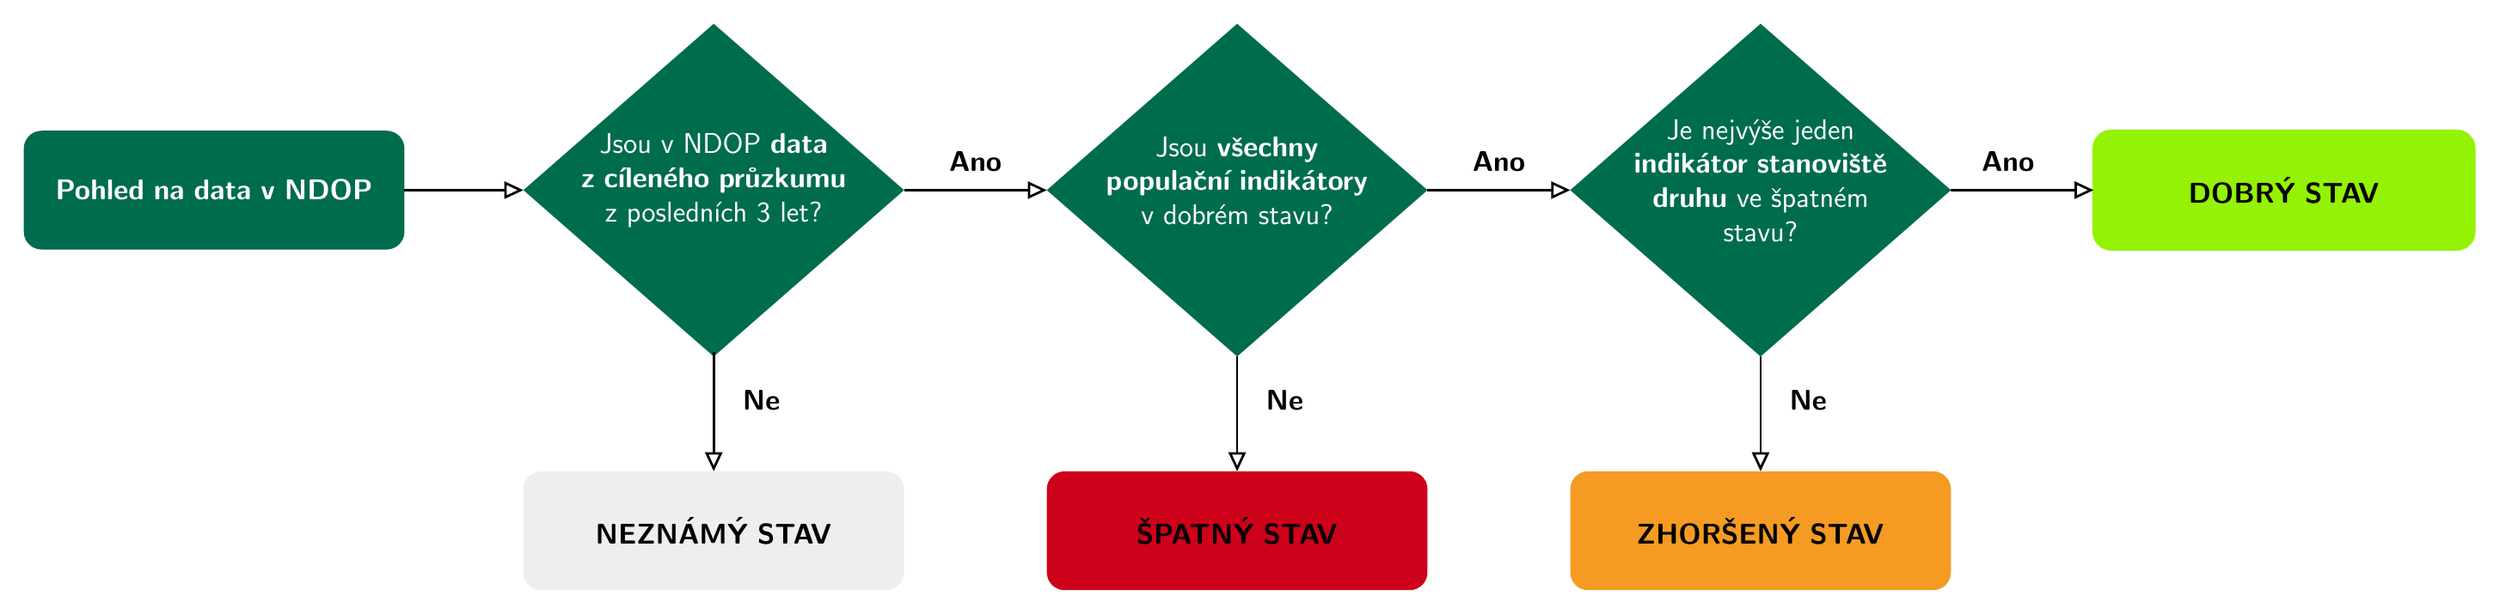
\begin{tikzpicture}[x=1.0000pt, y=-1.0000pt, line cap=butt, line join=miter]
  \path[fill=dio006C4E, draw=none, line width=1.00pt, rounded corners=7.50pt] (50.00,106.67) rectangle (210.00,156.67);
  \node[align=center, inner sep=0pt, outer sep=0pt, text=dioFFFFFF, font=\fontsize{12.00}{14.40}\selectfont, text width=156.00pt] at (130.00,131.67) {\textbf{Pohled na data v NDOP}};
  \path[fill=dio006C4E, draw=none, line width=1.00pt] (560.00,61.67) -- (640.00,131.67) -- (560.00,201.67) -- (480.00,131.67) -- cycle;
  \node[align=center, inner sep=0pt, outer sep=0pt, text=dioFFFFFF, font=\fontsize{12.00}{14.40}\selectfont, text width=148.00pt] at (560.00,127.67) {Jsou~\textbf{všechny}\\\textbf{populační indikátory}\\v dobrém stavu?};
  \path[fill=dio006C4E, draw=none, line width=1.00pt] (780.00,61.67) -- (860.00,131.67) -- (780.00,201.67) -- (700.00,131.67) -- cycle;
  \node[align=center, inner sep=0pt, outer sep=0pt, text=dioFFFFFF, font=\fontsize{12.00}{14.40}\selectfont, text width=148.00pt] at (780.00,127.67) {Je nejvýše jeden\\\textbf{indikátor stanoviště druhu} ve špatném\\stavu?};
  \path[fill=dioCD011A, draw=none, line width=1.00pt, rounded corners=7.50pt] (480.00,250.00) rectangle (640.00,300.00);
  \node[align=center, inner sep=0pt, outer sep=0pt, text=dio000000, font=\fontsize{12.00}{14.40}\selectfont, text width=156.00pt] at (560.00,275.00) {\textbf{ŠPATNÝ STAV}};
  \path[fill=dioF59B23, draw=none, line width=1.00pt, rounded corners=7.50pt] (700.00,250.00) rectangle (860.00,300.00);
  \node[align=center, inner sep=0pt, outer sep=0pt, text=dio000000, font=\fontsize{12.00}{14.40}\selectfont, text width=156.00pt] at (780.00,275.00) {\textbf{ZHORŠENÝ STAV}};
  \path[fill=dio94F204, draw=dio94F204, line width=1.00pt, rounded corners=7.50pt] (920.00,106.67) rectangle (1080.00,156.67);
  \node[align=center, inner sep=0pt, outer sep=0pt, text=dio000000, font=\fontsize{12.00}{14.40}\selectfont, text width=156.00pt] at (1000.00,131.67) {\textbf{DOBRÝ STAV}};
  \path[fill=dio006C4E, draw=none, line width=1.00pt] (340.00,61.67) -- (420.00,131.67) -- (340.00,201.67) -- (260.00,131.67) -- cycle;
  \node[align=center, inner sep=0pt, outer sep=0pt, text=dioFFFFFF, font=\fontsize{12.00}{14.40}\selectfont, text width=148.00pt] at (340.00,127.67) {Jsou v NDOP \textbf{data}\\\textbf{z cíleného průzkumu}\\z posledních 3 let?};
  \path[fill=dioEFEEED, draw=none, line width=1.00pt, rounded corners=7.50pt] (260.00,250.00) rectangle (420.00,300.00);
  \node[align=center, inner sep=0pt, outer sep=0pt, text=dio000000, font=\fontsize{12.00}{14.40}\selectfont, text width=156.00pt] at (340.00,275.00) {\textbf{NEZNÁMÝ STAV}};
  \draw[draw=dio000000, line width=1.00pt, -{Triangle[length=8.00pt, width=7.20pt, color=dio000000, fill=white, line width=1.00pt]}] (640.00,131.67) -- (700.00,131.67);
  \node[align=center, inner sep=0pt, outer sep=0pt, text=dio000000, font=\fontsize{12.00}{14.40}\selectfont] at (670.00,119.67) {\textbf{Ano}};
  \draw[draw=dio000000, line width=1.00pt, -{Triangle[length=8.00pt, width=7.20pt, color=dio000000, fill=white, line width=1.00pt]}] (560.00,201.67) -- (560.00,250.00);
  \node[align=center, inner sep=0pt, outer sep=0pt, text=dio000000, font=\fontsize{12.00}{14.40}\selectfont] at (580.00,220.00) {\textbf{Ne}};
  \draw[draw=dio000000, line width=1.00pt, -{Triangle[length=8.00pt, width=7.20pt, color=dio000000, fill=white, line width=1.00pt]}] (780.00,201.67) -- (780.00,250.00);
  \node[align=center, inner sep=0pt, outer sep=0pt, text=dio000000, font=\fontsize{12.00}{14.40}\selectfont] at (800.00,220.00) {\textbf{Ne}};
  \draw[draw=dio000000, line width=1.00pt, -{Triangle[length=8.00pt, width=7.20pt, color=dio000000, fill=white, line width=1.00pt]}] (860.00,131.67) -- (920.00,131.67);
  \node[align=center, inner sep=0pt, outer sep=0pt, text=dio000000, font=\fontsize{12.00}{14.40}\selectfont] at (884.00,119.67) {\textbf{Ano}};
  \draw[draw=dio000000, line width=1.00pt, -{Triangle[length=8.00pt, width=7.20pt, color=dio000000, fill=white, line width=1.00pt]}] (420.00,131.67) -- (480.00,131.67);
  \node[align=center, inner sep=0pt, outer sep=0pt, text=dio000000, font=\fontsize{12.00}{14.40}\selectfont] at (450.00,119.67) {\textbf{Ano}};
  \draw[draw=dio000000, line width=1.00pt, -{Triangle[length=8.00pt, width=7.20pt, color=dio000000, fill=white, line width=1.00pt]}] (210.00,131.67) -- (260.00,131.67);
  \draw[draw=dio000000, line width=1.00pt, -{Triangle[length=8.00pt, width=7.20pt, color=dio000000, fill=white, line width=1.00pt]}] (340.00,200.00) -- (340.00,250.00);
  \node[align=center, inner sep=0pt, outer sep=0pt, text=dio000000, font=\fontsize{12.00}{14.40}\selectfont] at (360.00,220.00) {\textbf{Ne}};
\end{tikzpicture}
\end{document}
